\chapter{Proposta: Estudo de Caso do Aplicativo InLight}
\label{sec:proposta}

Este capítulo apresenta o estudo de caso que constitui o Aplicativo InLight. A Seção~\ref{sec:metodologia} descreve a metodologia da pesquisa; a Seção~\ref{sec:contexto} apresenta o contexto do caso e o cenário atual de trabalho; a Seção~\ref{sec:inlight} descreve o aplicativo InLight, sua arquitetura e suas tecnologias; a Seção~\ref{sec:implantacao} propõe o processo com o aplicativo e um plano de implantação; a Seção~\ref{sec:avaliacao} define como a proposta será avaliada; e a Seção~\ref{sec:limitacoes} discute as limitações do estudo.

\section{Metodologia da Pesquisa}
\label{sec:metodologia}

\subsection{Classificação da Pesquisa}

Quanto à natureza, esta pesquisa é aplicada, pois busca gerar conhecimento para a solução de um problema concreto de uma organização. Quanto aos objetivos, é exploratória e descritiva: exploratória por tratar de um tema pouco estudado no contexto específico do ambiente regulado de energia, e descritiva por caracterizar o processo atual e a solução proposta \citep{gil2019}. A abordagem é mista, combinando dados qualitativos, como documentos e entrevistas, com dados quantitativos, como tempos de execução de tarefas e respostas a um questionário em escala.

Quanto ao procedimento, adota-se o estudo de caso único. Segundo \citet{yin2015}, o estudo de caso é adequado quando as questões de pesquisa são do tipo ``como'' e ``por que'', quando o pesquisador tem pouco controle sobre os eventos e quando o foco é um fenômeno contemporâneo em seu contexto real. As quatro questões de pesquisa deste trabalho atendem a essas condições.

\subsection{Fontes de Evidência e Triangulação}

\citet{yin2015} identifica seis fontes de evidência para estudos de caso: documentação, registros em arquivo, entrevistas, observação direta, observação participante e artefatos físicos. Este estudo utiliza quatro delas:

\begin{itemize}
    \item \textbf{Documentação:} documentos institucionais não confidenciais sobre o processo do BackOffice ACR;
    \item \textbf{Observação direta:} acompanhamento da execução das tarefas, com registro de tempos e etapas;
    \item \textbf{Questionário e entrevistas:} aplicados a usuários e gestores para captar sua percepção sobre o aplicativo;
    \item \textbf{Artefato:} o próprio aplicativo InLight, analisado quanto às suas funcionalidades e à sua arquitetura.
\end{itemize}

O uso de múltiplas fontes permite a triangulação dos dados, que, segundo \citet{yin2015}, fortalece a validade do estudo de caso, pois uma mesma conclusão passa a ser sustentada por evidências de origens diferentes. A Tabela~\ref{tab:matriz-questoes} relaciona cada questão de pesquisa às fontes de evidência e à base teórica que orienta sua análise.

\begin{table}[H]
\centering
\caption{Matriz de questões de pesquisa, fontes de evidência e base teórica}
\label{tab:matriz-questoes}
\footnotesize
\begin{tabularx}{\textwidth}{P{4.3cm}XX}
\toprule
\textbf{Questão de pesquisa} & \textbf{Fontes de evidência} & \textbf{Base teórica} \\ \midrule
QP1: Como sistemas fragmentados impactam a eficiência operacional da empresa? & Documentação; observação do processo atual & Fragmentação e redundância \citep{elmasri2016,laudon2020}; custos e benefícios da integração \citep{goodhue1992} \\ \midrule
QP2: De que forma a unificação, por meio do InLight, contribui para a integração de processos e o fluxo de informações? & Artefato; comparação entre o processo atual e o proposto & Integração e unificação \citep{linthicum2000,hohpe2003}; reengenharia \citep{hammer1990} \\ \midrule
QP3: Como observar e mensurar os benefícios e as limitações da unificação? & Indicadores de processo; questionário & Dimensões de desempenho \citep{dumas2018}; sucesso de SI \citep{delone2003}; benefícios \citep{shang2002} \\ \midrule
QP4: Como a visão de usuários e gestores influencia a adoção de sistemas unificados? & Questionário; entrevistas com gestores & TAM \citep{davis1989}; UTAUT \citep{venkatesh2003}; fatores críticos \citep{nah2001} \\ \bottomrule
\end{tabularx}

\vspace{0.2cm}
{\footnotesize Fonte: elaborado pelo autor.}
\end{table}

\subsection{Etapas da Pesquisa}

A pesquisa foi organizada nas etapas apresentadas na Figura~\ref{fig:etapas-pesquisa}. As duas primeiras correspondem aos Capítulos~\ref{sec:fundamentacao} e~\ref{sec:revisao}, as demais são desenvolvidas neste capítulo.

\begin{figure}[H]
\centering
\caption{Etapas da pesquisa}
\label{fig:etapas-pesquisa}
\begin{tikzpicture}[
    node distance=0.4cm,
    etapa/.style={rectangle, rounded corners=2pt, draw, thick, fill=gray!10,
                  text width=3.8cm, minimum height=1.1cm, align=center, font=\small},
    seta/.style={-{Stealth[length=2.5mm]}, thick}
]
\node[etapa] (e1) {1. Fundamentação\\teórica};
\node[etapa, right=of e1] (e2) {2. Revisão\\da literatura};
\node[etapa, right=of e2] (e3) {3. Diagnóstico\\do cenário atual};
\node[etapa, below=0.8cm of e3] (e4) {4. Descrição\\do InLight};
\node[etapa, left=of e4] (e5) {5. Processo proposto\\e plano de implantação};
\node[etapa, left=of e5] (e6) {6. Avaliação:\\indicadores e percepção};
\node[etapa, below=0.8cm of e6] (e7) {7. Análise\\e conclusões};
\draw[seta] (e1) -- (e2);
\draw[seta] (e2) -- (e3);
\draw[seta] (e3) -- (e4);
\draw[seta] (e4) -- (e5);
\draw[seta] (e5) -- (e6);
\draw[seta] (e6) -- (e7);
\end{tikzpicture}

\vspace{0.2cm}
{\footnotesize Fonte: elaborado pelo autor.}
\end{figure}

\subsection{Aspectos Éticos}

A coleta de dados utiliza apenas documentos institucionais disponibilizados para a pesquisa, sem acesso a informações confidenciais. A participação no questionário e nas entrevistas é voluntária, e as respostas são tratadas de forma anônima e agregada, de modo que nenhum participante possa ser identificado \citep{gil2019}.

\section{Contexto do Caso}
\label{sec:contexto}

\subsection{A Organização e a Área Estudada}

A Light é uma concessionária de distribuição de energia elétrica que atua no estado do Rio de Janeiro. Como distribuidora, adquire no Ambiente de Contratação Regulada a energia destinada ao atendimento de seus consumidores cativos, por meio dos contratos descritos na Seção~\ref{sec:setor}.

Segundo as informações financeiras intermediárias do segundo trimestre de 2026, divulgadas ao mercado \citep{light2026itr}, a Light Serviços de Eletricidade S.A. (Light SESA) é uma sociedade por ações de capital aberto, com sede na cidade do Rio de Janeiro, integralmente controlada pela Light S.A. Sua concessão de distribuição foi efetivada em julho de 1996 e, com o 8º Termo Aditivo, assinado em 6 de maio de 2026, foi prorrogada até 4 de junho de 2056. A área de concessão abrange 31 municípios do estado, incluindo a capital, com cerca de 4,2 milhões de unidades consumidoras faturadas, correspondentes a uma população de cerca de 10 milhões de pessoas. A energia destinada a esse mercado é adquirida de Itaipu Binacional, por meio de seu agente comercializador, a ENBPar, em leilões de energia existente, da CCEE e do Programa de Incentivo às Fontes Alternativas de Energia Elétrica (PROINFA).

A mesma fonte evidencia a relevância da compra de energia para a distribuidora. No primeiro semestre de 2026, os custos com energia elétrica somaram cerca de R\$~4,6 bilhões, dos quais cerca de R\$~2,1 bilhões referem-se a energia de leilões, frente a uma receita operacional líquida de cerca de R\$~6,9 bilhões. A companhia informa ainda compromissos de compra de energia em contratos de longo prazo superiores a R\$~6 bilhões por ano entre 2027 e 2031 e uma estratégia de contratação que busca manter o nível contratado entre 100\% e 105\% da energia requerida pelo mercado cativo, faixa associada ao limite regulatório para repasse da sobrecontratação às tarifas \citep{light2026itr}.

O estudo concentra-se no BackOffice de compra de energia do ACR, área responsável pelo acompanhamento dos contratos de compra de energia da distribuidora. Entre suas atividades estão o controle das notas dos contratos por quantidade, por disponibilidade e de cotas, com seus respectivos blocos; o acompanhamento de metas da área; e o tratamento de pagamentos que, pela forma como são processados, são denominados especiais. Atualmente, a equipe é composta de 5 integrantes: 1 coordenador, 3 analistas e 1 estagiário, este grupo é responsável pela administração de 522 contratos regulados, que se dividem em três blocos, além das Obrigações Setoriais que as distribuidoras tem que possuir e administrar.

\subsection{Cenário Atual}

No cenário anterior ao InLight, as informações necessárias a essas atividades estão distribuídas entre diferentes fontes: os sistemas da CCEE, a plataforma Thunders, um sistema de lançamento de notas cuja base de dados não é automatizada de forma completa aos demais sistemas corporativos, e controles mantidos em planilhas. A Figura~\ref{fig:as-is} representa, de forma simplificada, esse cenário: o analista precisa consultar cada fonte separadamente e consolidar as informações manualmente.

\begin{figure}[H]
\centering
\caption{Representação simplificada do cenário atual}
\label{fig:as-is}
\begin{tikzpicture}[
    fonte/.style={rectangle, rounded corners=2pt, draw, thick, fill=gray!10,
                  text width=2.8cm, minimum height=1cm, align=center, font=\small},
    ator/.style={ellipse, draw, thick, fill=blue!8, minimum width=2.6cm,
                 minimum height=1cm, align=center, font=\small},
    seta/.style={{Stealth[length=2.5mm]}-{Stealth[length=2.5mm]}, thick}
]
\node[ator] (analista) at (0,0) {Analista do\\BackOffice ACR};
\node[fonte] (ccee) at (-4.5,1.6) {Sistemas da CCEE};
\node[fonte] (thunders) at (4.5,1.6) {Plataforma Thunders};
\node[fonte] (notas) at (-4.5,-1.6) {Sistema de lançamento de notas};
\node[fonte] (planilhas) at (4.5,-1.6) {Planilhas de controle};
\node[fonte, fill=orange!15, text width=4.2cm] (consol) at (0,-3.2) {Consolidação manual\\(conferência e redigitação)};
\draw[seta] (analista) -- (ccee);
\draw[seta] (analista) -- (thunders);
\draw[seta] (analista) -- (notas);
\draw[seta] (analista) -- (planilhas);
\draw[-{Stealth[length=2.5mm]}, thick, dashed] (analista) -- (consol);
\end{tikzpicture}

\vspace{0.2cm}
{\footnotesize Fonte: elaborado pelo autor.}
\end{figure}

Na perspectiva da fundamentação teórica, apresenta as condições típicas da fragmentação de sistemas discutidas na Seção~\ref{sec:legados}. A Tabela~\ref{tab:problemas} relaciona os problemas descritos na literatura à forma como podem se manifestar no BackOffice ACR. Essas manifestações são tratadas como hipóteses a serem confirmadas pela análise documental e pela observação do processo.

\begin{table}[H]
\centering
\caption{Problemas da fragmentação e sua possível manifestação no caso}
\label{tab:problemas}
\footnotesize
\begin{tabularx}{\textwidth}{P{3.2cm}XP{3.2cm}}
\toprule
\textbf{Problema} & \textbf{Possível manifestação no BackOffice ACR} & \textbf{Base teórica} \\ \midrule
Redundância e inconsistência de dados & Dados de um mesmo contrato registrados em mais de uma fonte, com risco de versões divergentes & \citet{elmasri2016} \\ \midrule
Retrabalho e redigitação & Transcrição manual de informações da CCEE e da Thunders para planilhas e para o sistema de notas & \citet{stair2018}; \citet{hammer1990} \\ \midrule
Ausência de visão consolidada & Necessidade de reunir várias fontes para saber a situação dos contratos e dos próximos blocos & \citet{power2002}; \citet{sharda2014} \\ \midrule
Risco de descumprimento de prazos & Dependência de controles manuais para acompanhar vencimentos e pagamentos especiais & \citet{brasil2004decreto} \\ \midrule
Controle de acesso heterogêneo & Planilhas compartilhadas sem controle de permissões por perfil & \citet{whitman2018} \\ \bottomrule
\end{tabularx}

\vspace{0.2cm}
{\footnotesize Fonte: elaborado pelo autor.}
\end{table}

\section{O Aplicativo InLight}
\label{sec:inlight}

\subsection{Objetivo e Escopo}

O InLight é um aplicativo de unificação de sistemas desenvolvido para o BackOffice de compra de energia do ACR da Light. Seu objetivo é reunir em uma única aplicação as principais informações hoje distribuídas entre a CCEE, a plataforma Thunders e controles mantidos em planilhas. Embora tenha sido concebido para o mercado regulado, sua estrutura permite a ampliação para o mercado livre.

Em relação às estratégias descritas por \citet{bisbal1999}, o InLight não redesenvolve nem migra os sistemas existentes: estes continuam em operação e o aplicativo acrescenta uma nova camada que consolida as informações de que a área precisa. Na visão de \citet{linthicum2000}, trata-se de uma unificação nos níveis de dados e de interface do usuário, já que cria uma base de dados própria e uma interface única para as informações antes dispersas.

\subsection{Módulos}

O aplicativo está organizado em três módulos, descritos na Tabela~\ref{tab:modulos}, que também relaciona cada módulo aos problemas da Tabela~\ref{tab:problemas}.

\begin{table}[H]
\centering
\caption{Módulos do InLight}
\label{tab:modulos}
\footnotesize
\begin{tabularx}{\textwidth}{P{2cm}XX}
\toprule
\textbf{Módulo} & \textbf{Funcionalidades} & \textbf{Problemas endereçados} \\ \midrule
Notas & Agrupa os contratos por quantidade, por disponibilidade e de cotas, com todos os seus blocos; exibe na tela inicial um contador para o próximo bloco & Ausência de visão consolidada; risco de descumprimento de prazos; redundância de dados \\ \midrule
Metas & Permite o acompanhamento dinâmico de metas da área, com ajuste do progresso pelo usuário & Controles paralelos em planilhas; ausência de visão consolidada \\ \midrule
Obrigações & Trata os pagamentos especiais e permite importar obrigações futuras a partir de planilhas Excel, com validação dos dados & Retrabalho e redigitação; risco de descumprimento de prazos \\ \bottomrule
\end{tabularx}

\vspace{0.2cm}
{\footnotesize Fonte: elaborado pelo autor.}
\end{table}

As Figuras~\ref{fig:telas-acesso} a~\ref{fig:telas-metas} apresentam as telas principais do aplicativo, capturadas em ambiente de teste com dados fictícios. O acesso é feito por \textit{e-mail} e senha (Figura~\ref{fig:tela-login}); após a autenticação, o menu exibe um contador regressivo para o próximo vencimento e dá acesso à lista de pagamentos futuros, às notas, às metas e, no perfil de administrador, ao cadastro de usuários (Figura~\ref{fig:tela-menu}).

\begin{figure}[H]
    \centering
    \caption{Telas de acesso do InLight}
    \label{fig:telas-acesso}
    \subfloat[Tela de \textit{login}\label{fig:tela-login}]{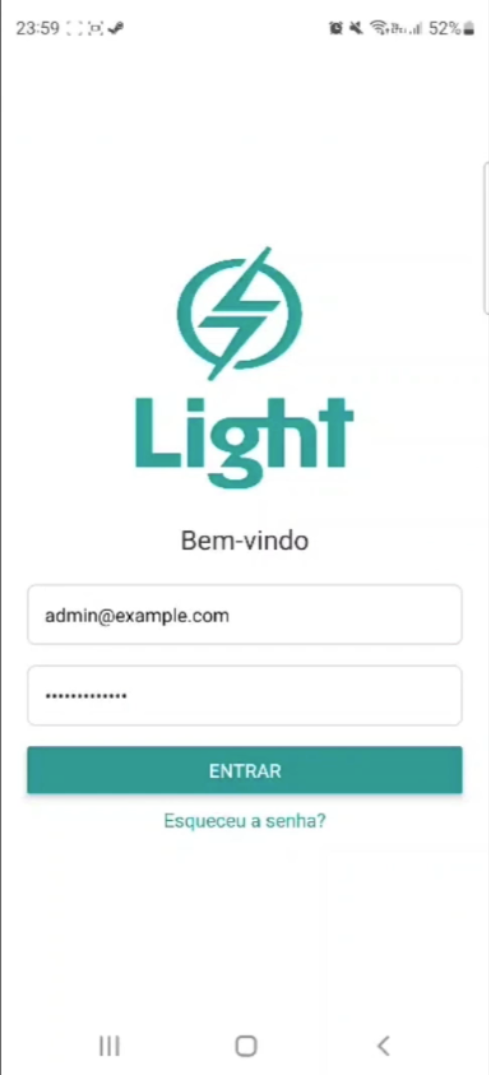
\includegraphics[width=0.38\textwidth]{Tela de Login.png}}
    \hspace{0.06\textwidth}
    \subfloat[Menu do administrador\label{fig:tela-menu}]{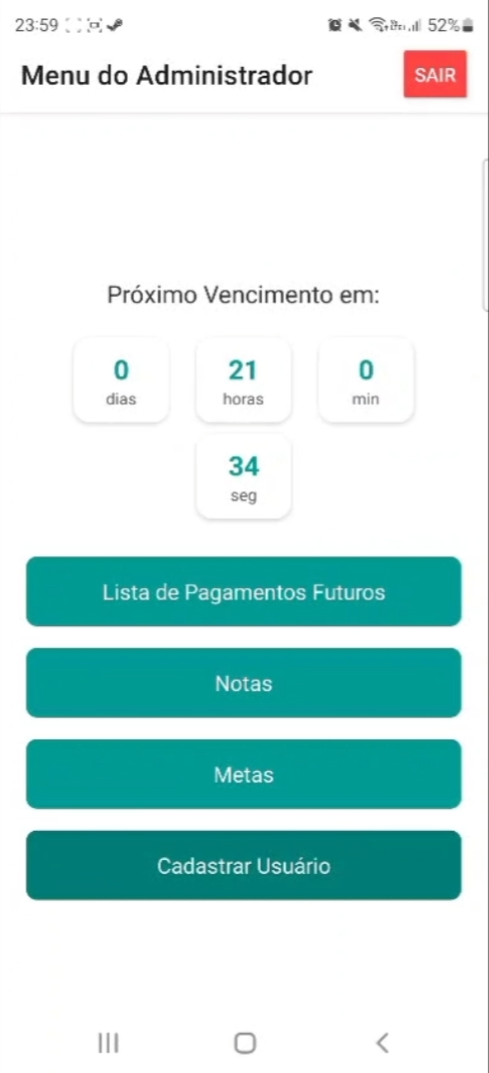
\includegraphics[width=0.38\textwidth]{Tela de Menu.png}}

    \vspace{0.2cm}
    {\footnotesize Fonte: elaborado pelo autor.}
\end{figure}

A Figura~\ref{fig:tela-pagamentos} mostra a lista de pagamentos futuros do módulo Obrigações. Cada obrigação apresenta a data de vencimento, a data de divulgação e os lembretes associados, e o botão ``Importar Excel'' permite carregar novas obrigações a partir de planilhas.

\begin{figure}[H]
    \centering
    \caption{Lista de pagamentos futuros do módulo Obrigações}
    \label{fig:tela-pagamentos}
    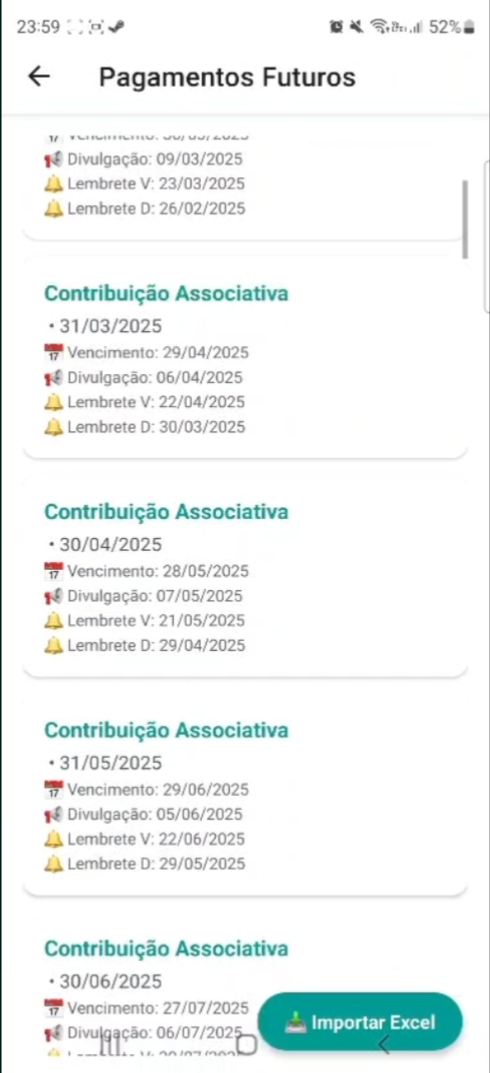
\includegraphics[width=0.38\textwidth]{Tela de Contratos.png}

    \vspace{0.2cm}
    {\footnotesize Fonte: elaborado pelo autor.}
\end{figure}

No módulo Metas, a equipe visualiza as metas cadastradas com seu percentual de conclusão (Figura~\ref{fig:tela-metas}) e, ao selecionar uma delas, consulta o criador, os responsáveis e o progresso, que pode ser ajustado pelo usuário (Figura~\ref{fig:tela-meta-detalhe}).

\begin{figure}[H]
    \centering
    \caption{Telas do módulo Metas}
    \label{fig:telas-metas}
    \subfloat[Lista de metas\label{fig:tela-metas}]{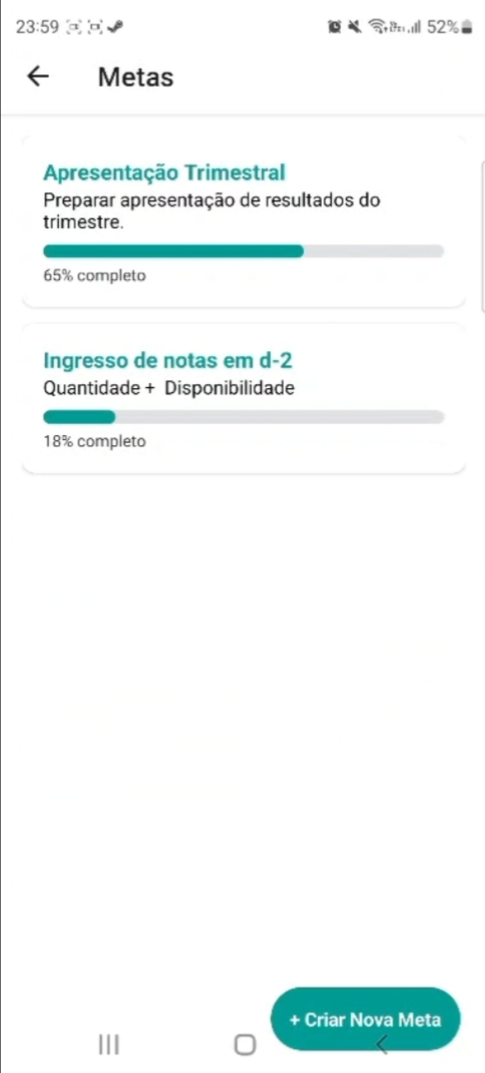
\includegraphics[width=0.38\textwidth]{Tela de Metas.png}}
    \hspace{0.06\textwidth}
    \subfloat[Detalhes de uma meta\label{fig:tela-meta-detalhe}]{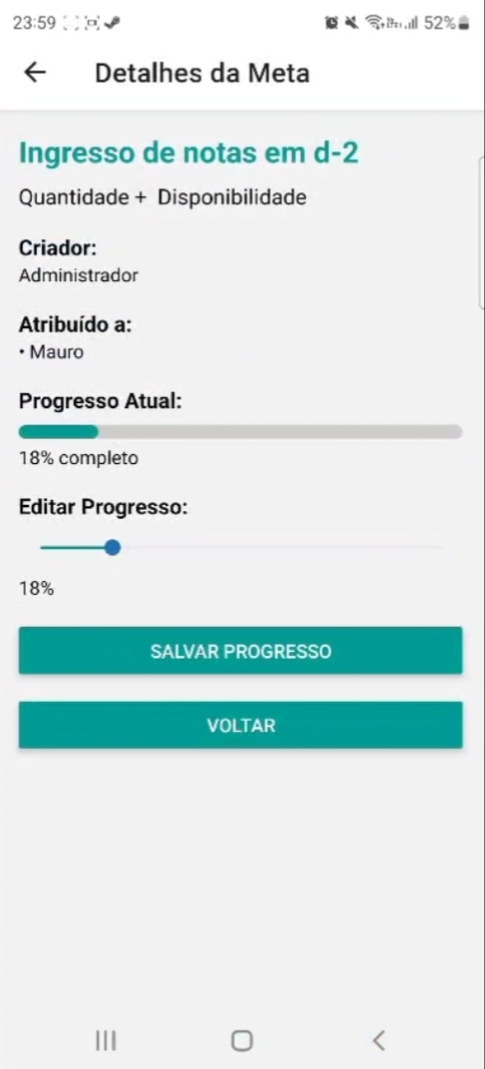
\includegraphics[width=0.38\textwidth]{Visao dentro de metas.png}}

    \vspace{0.2cm}
    {\footnotesize Fonte: elaborado pelo autor.}
\end{figure}

\subsection{Arquitetura}

O InLight adota uma arquitetura cliente-servidor, que separa a interface do usuário (\textit{front-end}) da lógica de negócio e do acesso a dados (\textit{back-end}). Segundo \citet{pressman2016}, essa separação facilita a manutenção e a escalabilidade e permite que equipes diferentes trabalhem em cada parte. A comunicação ocorre por meio de uma API que segue os princípios REST definidos por \citet{fielding2000}: separação entre cliente e servidor, ausência de estado entre requisições (\textit{stateless}), possibilidade de armazenamento em cache, interface uniforme e sistema em camadas. A Figura~\ref{fig:arquitetura} apresenta a visão geral da arquitetura.

\begin{figure}[H]
\centering
\caption{Visão geral da arquitetura do InLight}
\label{fig:arquitetura}
\begin{tikzpicture}[
    caixa/.style={rectangle, rounded corners=2pt, draw, thick, fill=gray!10,
                  text width=3.6cm, minimum height=0.9cm, align=center, font=\small},
    camada/.style={rectangle, draw, thick, fill=white,
                   text width=3.4cm, minimum height=0.75cm, align=center, font=\small},
    seta/.style={-{Stealth[length=2.5mm]}, thick},
    rotulo/.style={font=\scriptsize, align=center}
]
% Cliente
\node[caixa, fill=blue!8, text width=3.4cm, minimum height=2.4cm] (app) at (0,0)
    {\textbf{Aplicativo móvel}\\React Native + TypeScript\\[2pt]\scriptsize Context API, React Navigation, AsyncStorage};
% Servidor
\node[camada] (ctrl) at (6.2,1.1) {\textit{Controllers}};
\node[camada] (serv) at (6.2,0) {\textit{Services}};
\node[camada] (repo) at (6.2,-1.1) {\textit{Repositories} (TypeORM)};
\node[draw, thick, dashed, rounded corners=3pt, inner sep=6pt,
      fit=(ctrl)(serv)(repo), label={[font=\small\bfseries]above:API NestJS (Node.js)}] (api) {};
% Banco
\node[cylinder, shape border rotate=90, aspect=0.25, draw, thick, fill=gray!10,
      minimum width=2.4cm, minimum height=1.4cm, align=center, font=\small] (db) at (6.2,-3.5) {PostgreSQL};
% Planilhas
\node[caixa, text width=2.6cm] (xlsx) at (0,-3.5) {Planilhas (.xlsx)};
% Setas
\draw[seta] (app.east |- ctrl) -- node[rotulo, above] {HTTP/REST\\+ token JWT} (ctrl.west);
\draw[seta] (ctrl) -- (serv);
\draw[seta] (serv) -- (repo);
\draw[seta] (api.south) -- (db.north);
\draw[seta, dashed] (xlsx.north) -- node[rotulo, left] {importação} (app.south);
\end{tikzpicture}

\vspace{0.2cm}
{\footnotesize Fonte: elaborado pelo autor.}
\end{figure}

\subsection{Tecnologias Utilizadas}

A Tabela~\ref{tab:stack} resume as tecnologias empregadas, que são detalhadas a seguir.

\begin{table}[H]
\centering
\caption{Tecnologias utilizadas no InLight}
\label{tab:stack}
\footnotesize
\begin{tabularx}{\textwidth}{P{2.6cm}P{3.6cm}X}
\toprule
\textbf{Camada} & \textbf{Tecnologia} & \textbf{Função} \\ \midrule
Interface & React Native, TypeScript & Aplicativo multiplataforma (Android e iOS) com tipagem estática \\ \midrule
Servidor & NestJS, Node.js & API REST organizada em módulos e camadas \\ \midrule
Persistência & PostgreSQL, TypeORM & Armazenamento relacional e mapeamento objeto-relacional \\ \midrule
Segurança & JWT, Passport.js, bcrypt, RBAC & Autenticação, armazenamento seguro de senhas e controle de acesso por perfil \\ \midrule
Qualidade & \textit{class-validator}, Jest & Validação de dados de entrada e testes automatizados \\ \bottomrule
\end{tabularx}

\vspace{0.2cm}
{\footnotesize Fonte: elaborado pelo autor.}
\end{table}

\subsubsection{Front-end: React Native e TypeScript}

O \textit{front-end} foi desenvolvido em React Native, framework mantido pela Meta que permite criar aplicações para Android e iOS a partir de uma única base de código \citep{eisenman2015}. A escolha se justifica pelo desenvolvimento multiplataforma, que reduz tempo e custo, pelo recarregamento rápido do código durante o desenvolvimento e pela comunidade ativa, com ampla oferta de bibliotecas.

Todo o projeto utiliza TypeScript, linguagem que acrescenta tipagem estática opcional ao JavaScript. Segundo \citet{bierman2014}, essa tipagem permite detectar erros ainda durante o desenvolvimento e melhora o suporte das ferramentas, como o autocompletar e a refatoração \citep{microsoft2020}.

Para o estado global, utiliza-se a Context API do React, que compartilha dados entre componentes sem a necessidade de repassá-los manualmente por toda a árvore de componentes \citep{react2023}, o contexto de autenticação (AuthContext) gerencia o usuário conectado e seus tokens de acesso. A navegação entre telas usa a biblioteca React Navigation, no padrão \textit{Stack Navigator} \citep{reactnavigation2023}, e o armazenamento local de dados, como os tokens, usa o AsyncStorage, um armazenamento chave-valor assíncrono e não criptografado \citep{reactnative2023}. A interface é composta pelos componentes básicos do React Native, complementados por bibliotecas como \textit{@react-native-community/slider} (ajuste do progresso de metas), \textit{@react-native-picker/picker} (seleção de perfis de usuário) e \textit{expo-document-picker} (seleção de arquivos para \textit{upload}).

\subsubsection{Back-end: NestJS e Node.js}

O \textit{back-end} é desenvolvido em NestJS, framework para aplicações de servidor construído sobre o Node.js e que utiliza TypeScript como linguagem padrão, mantendo a mesma linguagem em toda a aplicação \citep{nestjs2023}. O NestJS oferece arquitetura modular, injeção de dependências e uso de \textit{decorators}, recursos que tornam o código mais organizado e testável.

O código segue uma arquitetura em camadas, conforme os padrões descritos por \citet{fowler2002}:

\begin{enumerate}
    \item \textbf{Apresentação (\textit{Controllers}):} recebe as requisições HTTP, valida as entradas e devolve as respostas, com rotas definidas por \textit{decorators} como @Get, @Post, @Patch e @Delete;
    \item \textbf{Negócio (\textit{Services}):} concentra as regras e validações do negócio e coordena as operações entre entidades;
    \item \textbf{Dados (\textit{Repositories}):} realiza a comunicação com o banco de dados, isolando os detalhes de persistência por meio do padrão \textit{Repository}.
\end{enumerate}

Essa separação aplica o princípio da responsabilidade única \citep{martin2008}. Os dados trafegam entre as camadas por meio de \textit{Data Transfer Objects} (DTOs), objetos simples que transportam dados sem conter lógica de negócio \citep{fowler2002}. A validação das entradas usa a biblioteca \textit{class-validator} em conjunto com o \textit{ValidationPipe} do NestJS, configurado para descartar propriedades não previstas no DTO, rejeitar requisições com campos extras e converter automaticamente os tipos primitivos. As respostas e os erros da API são padronizados por um \textit{ResponseInterceptor} e por um \textit{HttpExceptionFilter}, o que facilita o tratamento no \textit{front-end} \citep{nestjs2023}.

A importação de obrigações a partir de arquivos Excel (.xlsx) é feita por envio no formato \textit{multipart/\allowbreak form-data}. Nesse processo, as datas, que o Excel armazena como números seriais, são convertidas para o formato padrão, e os dados são validados antes de serem gravados, com retorno ao usuário sobre o sucesso ou os erros encontrados. Essa funcionalidade contribui para o princípio de capturar a informação uma única vez, defendido por \citet{hammer1990}, ao substituir a redigitação dos dados pela importação validada.

\subsubsection{Banco de Dados e Persistência}

O sistema gerenciador de banco de dados adotado é o PostgreSQL, de código aberto e conhecido pela confiabilidade e pela conformidade com o padrão SQL \citep{postgresql2023}. Segundo \citet{obe2017}, ele oferece suporte completo a transações ACID, tipos de dados extensíveis, índices avançados e suporte a dados em JSON.

O acesso ao banco é feito pelo TypeORM, ferramenta de mapeamento objeto-relacional (ORM) que permite manipular as tabelas como classes TypeScript e oferece construção de consultas, controle de versões do esquema (\textit{migrations}) e definição declarativa de relacionamentos \citep{typeorm2023}. O uso de um ORM reduz a quantidade de SQL escrito manualmente e facilita a portabilidade entre bancos de dados \citep{ambler2003}.

\subsubsection{Autenticação e Segurança}

A autenticação utiliza JSON Web Tokens (JWT), padrão aberto definido na RFC 7519 para a transmissão de informações entre as partes na forma de um objeto JSON assinado digitalmente \citep{jones2015}. O usuário envia suas credenciais, o servidor as valida e devolve um token, que o aplicativo armazena e envia nas requisições seguintes; como o token contém as informações necessárias, o servidor não precisa manter sessões. A validação do token é feita com a biblioteca Passport.js e sua estratégia \textit{passport-jwt}, integradas ao NestJS por meio de \textit{Guards} que protegem as rotas \citep{passport2023}.

As senhas são armazenadas com o algoritmo bcrypt, que aplica um \textit{salt} único a cada senha e possui custo computacional ajustável, o que dificulta ataques por tabelas pré-computadas e por força bruta \citep{provos1999}. Como o aplicativo e a API operam em origens diferentes, o \textit{back-end} também configura o CORS (\textit{Cross-Origin Resource Sharing}), definindo as origens e os métodos HTTP autorizados \citep{w3c2014}.

O controle de acesso segue o modelo baseado em papéis (RBAC), que, segundo \citet{ferraiolo2001}, simplifica a administração de permissões ao associá-las a papéis, e não a cada usuário individualmente. A Tabela~\ref{tab:perfis} apresenta os papéis definidos no InLight. Em comparação com planilhas compartilhadas, esse modelo permite aplicar uma política de acesso uniforme às informações da área \citep{whitman2018}.

\begin{table}[H]
\centering
\caption{Perfis de acesso do InLight}
\label{tab:perfis}
\footnotesize
\begin{tabularx}{\textwidth}{P{2.2cm}X}
\toprule
\textbf{Perfil} & \textbf{Permissões} \\ \midrule
Admin & Acesso total, incluindo o cadastro de usuários e a importação de dados \\ \midrule
Manager & Permissões de gestão sobre as informações da área \\ \midrule
User & Acesso às funcionalidades essenciais de consulta e acompanhamento \\ \bottomrule
\end{tabularx}

\vspace{0.2cm}
{\footnotesize Fonte: elaborado pelo autor.}
\end{table}

\subsubsection{Testes Automatizados}

Os testes utilizam o framework Jest, que permite escrever testes unitários e de integração, simular dependências externas (\textit{mocking}) e gerar relatórios de cobertura de código. O pacote \textit{@nestjs/testing} complementa o Jest ao facilitar a criação de módulos de teste com injeção de dependências \citep{nestjs2023}.

\section{Processo Proposto e Plano de Implantação}
\label{sec:implantacao}

\subsection{Processo com o InLight}

Com o InLight, o analista passa a consultar as informações dos contratos, metas e obrigações em uma única aplicação, como representado na Figura~\ref{fig:to-be}. As informações provenientes das fontes externas são registradas ou importadas uma vez no aplicativo, com validação na entrada, e passam a ser compartilhadas por toda a equipe conforme o perfil de acesso de cada usuário.

Na versão atual, o InLight não possui integração automática com os sistemas da CCEE nem com a plataforma Thunders. Os dados entram no aplicativo por registro ou por importação de planilhas no formato .xlsx, validadas antes da gravação. A integração por meio de API com essas duas fontes está prevista para versões futuras e depende da disponibilização das respectivas interfaces, que se encontra em andamento. Quando implementada, essa integração eliminará a etapa de importação manual e aproximará o InLight da integração no nível de interface de aplicação descrita por \citet{linthicum2000}.

\begin{figure}[H]
\centering
\caption{Representação simplificada do processo com o InLight}
\label{fig:to-be}
\begin{tikzpicture}[
    fonte/.style={rectangle, rounded corners=2pt, draw, thick, fill=gray!10,
                  text width=2.6cm, minimum height=0.9cm, align=center, font=\small},
    ator/.style={ellipse, draw, thick, fill=blue!8, minimum width=2.4cm,
                 minimum height=0.9cm, align=center, font=\small},
    seta/.style={-{Stealth[length=2.5mm]}, thick}
]
\node[rectangle, rounded corners=3pt, draw, very thick, fill=green!8,
      text width=3.4cm, minimum height=3.4cm, align=center, font=\small] (inlight) at (0,0)
      {\textbf{InLight}\\[4pt]Notas\\Metas\\Obrigações\\[4pt]\scriptsize base de dados única};
\node[fonte] (ccee) at (-6,1.2) {Sistemas da CCEE};
\node[fonte] (thunders) at (-6,0) {Plataforma Thunders};
\node[fonte] (planilhas) at (-6,-1.2) {Planilhas};
\node[ator] (analista) at (4.6,0.8) {Analista};
\node[ator] (gestor) at (4.6,-0.8) {Gestor};
\draw[seta, dashed] (ccee.east) -- (inlight.west |- ccee.east);
\draw[seta, dashed] (thunders.east) -- (inlight.west);
\draw[seta, dashed] (planilhas.east) -- (inlight.west |- planilhas.east);
\node[font=\scriptsize, align=center, above=0.1cm of ccee.north east, xshift=1.35cm] {registro ou\\importação (.xlsx)};
\node[font=\scriptsize, align=center, below=0.3cm of planilhas.south] {CCEE e Thunders: integração\\por API prevista};
\draw[{Stealth[length=2.5mm]}-{Stealth[length=2.5mm]}, thick] (inlight.east |- analista) -- (analista.west);
\draw[{Stealth[length=2.5mm]}-{Stealth[length=2.5mm]}, thick] (inlight.east |- gestor) -- (gestor.west);
\end{tikzpicture}

\vspace{0.2cm}
{\footnotesize Fonte: elaborado pelo autor.}
\end{figure}

Seguindo \citet{hammer1990} e \citet{dumas2018}, a mudança não deve se limitar a transferir os passos atuais para o aplicativo. Recomenda-se, na implantação, revisar o processo para eliminar etapas que deixam de ser necessárias, como a conferência de uma mesma informação em várias fontes e a manutenção de planilhas paralelas às informações registradas no InLight.

\subsection{Plano de Implantação}

O plano de implantação proposto segue as fases do ciclo de vida de sistemas corporativos definidas por \citet{markus2000}: concepção (\textit{chartering}), projeto (\textit{project}), estabilização (\textit{shakedown}) e evolução (\textit{onward and upward}). A Tabela~\ref{tab:plano} apresenta as atividades propostas para cada fase e os fatores críticos de sucesso de \citet{nah2001} a que elas respondem.

\begin{table}[H]
\centering
\caption{Plano de implantação proposto para o InLight}
\label{tab:plano}
\footnotesize
\begin{tabularx}{\textwidth}{P{2.5cm}XP{4cm}}
\toprule
\textbf{Fase} & \textbf{Atividades propostas} & \textbf{Fatores críticos relacionados} \\ \midrule
Concepção & Definir objetivos e indicadores; mapear o processo atual & Apoio da alta direção; plano e visão de negócio \\ \midrule
Projeto & Validar os módulos com os usuários-chave; carregar e conferir os dados iniciais; redesenhar o processo; capacitar a equipe & Composição da equipe; redesenho de processos; testes; comunicação eficaz \\ \midrule
Estabilização & Operar com acompanhamento próximo; registrar e corrigir problemas; desativar gradualmente as planilhas paralelas & Gestão da mudança; monitoramento e avaliação de desempenho \\ \midrule
Evolução & Medir os indicadores após o período de adaptação; priorizar melhorias; avaliar a extensão ao mercado livre & Monitoramento e avaliação de desempenho; defensor do projeto \\ \bottomrule
\end{tabularx}

\vspace{0.2cm}
{\footnotesize Fonte: elaborado pelo autor com base em \citet{markus2000} e \citet{nah2001}.}
\end{table}

Para a gestão da mudança, adotam-se como referência as recomendações de \citet{kotter1996}, em especial criar senso de urgência, comunicar com clareza a visão da mudança e gerar ganhos de curto prazo visíveis. No caso do InLight, um ganho de curto prazo pode ser a substituição de um controle em planilha que hoje exige mais esforço da equipe, cujo resultado seja percebido rapidamente pelos usuários.

\section{Avaliação da Proposta}
\label{sec:avaliacao}

\subsection{Desenho da Avaliação}

A avaliação combina duas perspectivas, conforme recomendado pela literatura revisada no Capítulo~\ref{sec:revisao} \citep{petter2008,wixom2005}: (i) indicadores de processo, que comparam o cenário atual com o cenário com o InLight e (ii) a percepção de usuários e gestores. Os resultados são, então, organizados segundo as dimensões de benefícios de \citet{shang2002}.

Como os benefícios de sistemas integrados podem demorar a aparecer e o desempenho pode cair logo após a implantação \citep{hitt2002,markus2000learning}, propõe-se medir os indicadores em dois momentos após a implantação: ao final da fase de estabilização e após um período de uso regular.

\subsection{Indicadores de Processo}

Os indicadores foram definidos a partir das quatro dimensões de desempenho de \citet{dumas2018}: tempo, custo, qualidade e flexibilidade. Para cada indicador, devem ser selecionadas tarefas representativas do BackOffice, executadas no cenário atual e com o InLight. A Tabela~\ref{tab:indicadores} apresenta os indicadores propostos.

\begin{table}[H]
\centering
\caption{Indicadores de processo propostos}
\label{tab:indicadores}
\footnotesize
\begin{tabularx}{\textwidth}{P{3.4cm}XP{1.9cm}P{2.6cm}}
\toprule
\textbf{Indicador} & \textbf{Definição operacional} & \textbf{Dimensão} & \textbf{Coleta} \\ \midrule
Tempo de consolidação & Tempo para reunir as informações necessárias sobre a situação de um contrato ou bloco & Tempo & Observação direta (cronometragem) \\ \midrule
Fontes consultadas & Número de sistemas e arquivos consultados para concluir uma tarefa & Tempo & Observação direta \\ \midrule
Redigitações & Número de vezes que um mesmo dado é digitado em fontes diferentes & Custo & Observação e documentação \\ \midrule
Inconsistências & Número de divergências encontradas entre fontes em uma conferência & Qualidade & Documentação \\ \midrule
Cumprimento de prazos & Proporção de obrigações e pagamentos especiais tratados dentro do prazo & Qualidade & Registros da área \\ \midrule
Erros de importação & Proporção de registros rejeitados pela validação na importação de planilhas & Qualidade & Registros do InLight \\ \midrule
Adaptação a novas demandas & Tempo para disponibilizar uma nova funcionalidade solicitada pela área & Flexibilidade & Histórico do projeto \\ \bottomrule
\end{tabularx}

\vspace{0.2cm}
{\footnotesize Fonte: elaborado pelo autor com base em \citet{dumas2018}.}
\end{table}

\subsection{Percepção dos Usuários}

A percepção dos usuários será medida por um questionário aplicado a todos os usuários do InLight no BackOffice ACR. Os itens de utilidade percebida e de facilidade de uso percebida foram adaptados do instrumento validado por \citet{davis1989}; os itens de qualidade da informação e de satisfação foram elaborados com base nas dimensões de \citet{delone2003}. As respostas serão coletadas em escala de sete pontos, de ``discordo totalmente'' a ``concordo totalmente''. A Tabela~\ref{tab:questionario} apresenta os itens.

\begin{table}[H]
\centering
\caption{Itens do questionário de percepção dos usuários}
\label{tab:questionario}
\footnotesize
\begin{tabularx}{\textwidth}{P{1.2cm}X}
\toprule
\textbf{Código} & \textbf{Item} \\ \midrule
\multicolumn{2}{l}{\textit{Utilidade percebida, adaptado de \citet{davis1989}}} \\ \midrule
UP1 & Usar o InLight me permite realizar minhas tarefas mais rapidamente. \\ \midrule
UP2 & Usar o InLight melhora meu desempenho no trabalho. \\ \midrule
UP3 & Usar o InLight aumenta minha produtividade. \\ \midrule
UP4 & Usar o InLight aumenta minha eficácia no trabalho. \\ \midrule
UP5 & Usar o InLight torna meu trabalho mais fácil. \\ \midrule
UP6 & Considero o InLight útil no meu trabalho. \\ \midrule
\multicolumn{2}{l}{\textit{Facilidade de uso percebida, adaptado de \citet{davis1989}}} \\ \midrule
FU1 & Aprender a operar o InLight foi fácil para mim. \\ \midrule
FU2 & Acho fácil fazer o InLight realizar o que preciso. \\ \midrule
FU3 & Minha interação com o InLight é clara e compreensível. \\ \midrule
FU4 & Considero o InLight flexível para interagir. \\ \midrule
FU5 & Foi fácil tornar-me habilidoso no uso do InLight. \\ \midrule
FU6 & Considero o InLight fácil de usar. \\ \midrule
\multicolumn{2}{l}{\textit{Qualidade da informação e satisfação, com base em \citet{delone2003}}} \\ \midrule
QI1 & As informações apresentadas pelo InLight são precisas. \\ \midrule
QI2 & As informações apresentadas pelo InLight estão atualizadas. \\ \midrule
QI3 & O InLight reúne as informações de que preciso sem que eu tenha de consultar outras fontes. \\ \midrule
SU1 & De modo geral, estou satisfeito com o InLight. \\ \bottomrule
\end{tabularx}

\vspace{0.2cm}
{\footnotesize Fonte: elaborado pelo autor, com itens adaptados de \citet{davis1989}.}
\end{table}

Para captar a visão dos gestores, propõe-se uma entrevista semiestruturada baseada nos determinantes da UTAUT \citep{venkatesh2003} e nos fatores críticos de \citet{nah2001}, com as perguntas da Tabela~\ref{tab:roteiro}.

\begin{table}[H]
\centering
\caption{Roteiro de entrevista com gestores}
\label{tab:roteiro}
\footnotesize
\begin{tabularx}{\textwidth}{P{3.6cm}X}
\toprule
\textbf{Construto} & \textbf{Pergunta} \\ \midrule
Expectativa de desempenho & Que ganhos o senhor ou a senhora espera, ou já percebe, no trabalho da equipe com o InLight? \\ \midrule
Expectativa de esforço & Quais dificuldades a equipe encontrou ou pode encontrar para usar o aplicativo? \\ \midrule
Influência social & De que forma a gestão incentiva o uso do InLight no lugar das planilhas? \\ \midrule
Condições facilitadoras & Que recursos, como treinamento, suporte e infraestrutura, estão disponíveis para apoiar o uso? \\ \midrule
Apoio da alta direção & Como a direção da área acompanha e apoia a implantação? \\ \midrule
Benefícios e limitações & Que benefícios e que limitações o senhor ou a senhora identifica na unificação das informações? \\ \bottomrule
\end{tabularx}

\vspace{0.2cm}
{\footnotesize Fonte: elaborado pelo autor com base em \citet{venkatesh2003} e \citet{nah2001}.}
\end{table}

\subsection{Benefícios Esperados por Dimensão}

A Tabela~\ref{tab:beneficios} organiza os benefícios esperados com o InLight segundo as dimensões de \citet{shang2002} e indica como cada um será verificado. Trata-se de hipóteses de trabalho, que serão confirmadas ou refutadas pelos resultados.

\begin{table}[H]
\centering
\caption{Benefícios esperados com o InLight por dimensão}
\label{tab:beneficios}
\footnotesize
\begin{tabularx}{\textwidth}{P{2.6cm}XP{3.6cm}}
\toprule
\textbf{Dimensão} & \textbf{Benefício esperado} & \textbf{Como verificar} \\ \midrule
Operacional & Redução do tempo de consolidação e do retrabalho & Tempo de consolidação; redigitações \\ \midrule
Gerencial & Visão consolidada dos contratos, metas e obrigações para a tomada de decisão & Entrevistas com gestores; item QI3 \\ \midrule
Estratégica & Base para a extensão ao mercado livre & Entrevistas com gestores \\ \midrule
Infraestrutura de TI & Plataforma modular, com controle de acesso uniforme & Análise do artefato; tempo de adaptação a novas demandas \\ \midrule
Organizacional & Redução da dependência de controles individuais em planilhas & Questionário; entrevistas \\ \bottomrule
\end{tabularx}

\vspace{0.2cm}
{\footnotesize Fonte: elaborado pelo autor com base em \citet{shang2002}.}
\end{table}

\subsection{Resultados}

Até a conclusão desta etapa do trabalho, o InLight ainda não foi implantado no BackOffice ACR. Por esse motivo, os indicadores da Tabela~\ref{tab:indicadores} não foram medidos, e o questionário e as entrevistas ainda não foram aplicados. A Tabela~\ref{tab:resultados} apresenta a estrutura em que os resultados serão registrados, comparando o cenário atual com o cenário com o InLight. Os benefícios da Tabela~\ref{tab:beneficios} permanecem, portanto, como hipóteses de trabalho, a serem confirmadas ou refutadas após a implantação, nos momentos de medição definidos no desenho da avaliação.


\begin{table}[H]
\centering
\caption{Resultados dos indicadores de processo}
\label{tab:resultados}
\footnotesize
\begin{tabularx}{\textwidth}{Xccc}
\toprule
\textbf{Indicador} & \textbf{Cenário atual} & \textbf{Com o InLight} & \textbf{Variação} \\ \midrule
Tempo de consolidação & --- & --- & --- \\ \midrule
Fontes consultadas & --- & --- & --- \\ \midrule
Redigitações & --- & --- & --- \\ \midrule
Inconsistências & --- & --- & --- \\ \midrule
Cumprimento de prazos & --- & --- & --- \\ \midrule
Erros de importação & --- & --- & --- \\ \midrule
Adaptação a novas demandas & --- & --- & --- \\ \bottomrule
\end{tabularx}

\vspace{0.2cm}
{\footnotesize Fonte: dados da pesquisa.}
\end{table}

\section{Limitações e Ameaças à Validade}
\label{sec:limitacoes}

Este estudo apresenta limitações que devem ser consideradas na interpretação dos resultados:

\begin{itemize}
    \item \textbf{Caso único:} os resultados não podem ser generalizados estatisticamente para outras organizações. Segundo \citet{yin2015}, estudos de caso permitem generalização analítica, isto é, a comparação dos resultados com a teoria, e não a extrapolação para uma população;
    \item \textbf{Momento da avaliação:} como o InLight ainda não foi implantado, os resultados dependem de medições futuras;
    \item \textbf{Número de participantes:} os respondentes se restringem aos usuários do InLight na área estudada, o que pode limitar o uso de técnicas estatísticas mais robustas na análise do questionário;
    \item \textbf{Proximidade do pesquisador:} o eventual envolvimento do pesquisador com a área ou com o desenvolvimento do aplicativo pode influenciar a coleta e a interpretação dos dados; para reduzir esse risco, utilizam-se múltiplas fontes de evidência e a triangulação \citep{yin2015};
    \item \textbf{Restrição de dados:} por não utilizar informações confidenciais, o estudo não analisa valores financeiros dos contratos.
\end{itemize}